\subsubsection{Container và GitOps (Docker, Kubernetes, ArgoCD)}

\begin{itemize}

\item \textbf{Docker:}
Hệ thống chạy tốt trên máy của lập trình viên
nhưng lỗi khi lên server do khác biệt về hệ điều hành hoặc thư viện.
Docker đóng gói ứng dụng cùng với các thư viện,
file cấu hình
và môi trường cần thiết vào một hộp kín gọi là Container.

\item \textbf{Kubernetes (K8s):}
Khi có nhiều container
trên các server khác nhau,
nếu một server down thì sao?
Nếu đột nhiên lượng truy cập tăng vọt thì làm thế nào?
Kubernetes là một hệ thống công cụ quản lý container (container orchestration).
Giúp tự động hóa việc triển khai, mở rộng quy mô và quản lý các container.
Kubernetes có khả năng thực hiện tính năng Rolling Update.
Đây là một trong những cơ chế đảm bảo không gián đoạn dịch vụ (Zero Downtime)
bằng cách tạo từ từ các Pod mới và lần lượt tắt các Pod cũ.
Kubernetes không xóa tất cả các Pod cùng một lúc.
Điều này đảm bảo ứng dụng luôn có Pod đang chạy để xử lý yêu cầu từ người dùng.

\item \textbf{GitOps với ArgoCD:}
Việc cấu hình hệ thống bằng cách gõ lệnh thủ công rất dễ dẫn đến sai sót,
khó theo dõi ai đã thay đổi gì
và cực kỳ khó khôi phục nếu hệ thống sập.
GitOps là một phương pháp sử dụng manifest của Git (như GitHub, GitLab)
là nguồn chân lý duy nhất (Single Source of Truth).
Các file yaml của K8s đều được lưu trên Git. ArgoCD nhận diện thay đổi và tự động triển khai (deploy) hoặc tinh chỉnh hạ tầng thực tế cho khớp với Git.

\end{itemize}

Docker image code-chatbot-service được đặt là private
vì image này quan trọng nhất của toàn bộ dự án.
Kết quả các Docker Image được push lên Docker Hub:

\begin{figure}[H]
\centering
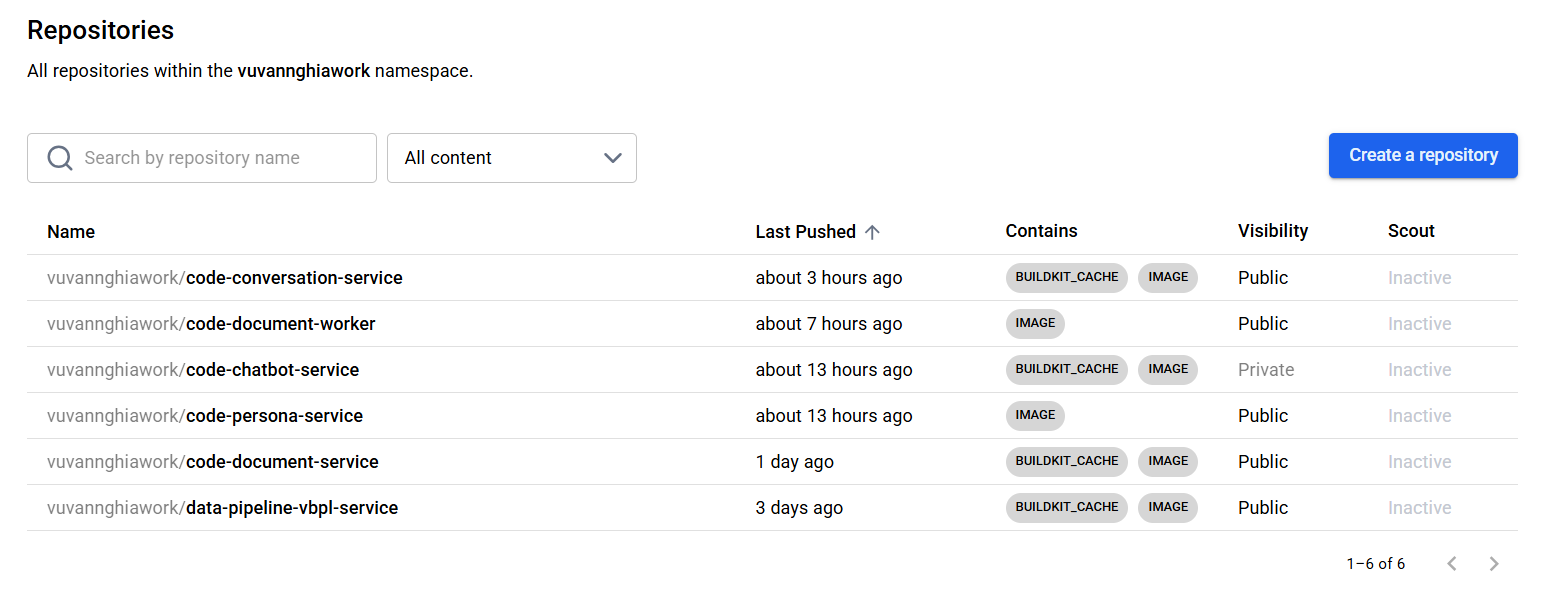
\includegraphics[width=0.95\textwidth]{pictures/docker-hub-web-ui2.png}
\caption{Kết quả các Docker Image được push lên Docker Hub}
\end{figure}

Kết quả giao diện ArgoCD chạy triển khai các docker iamge trong kubernetes:

\begin{figure}[H]
\centering
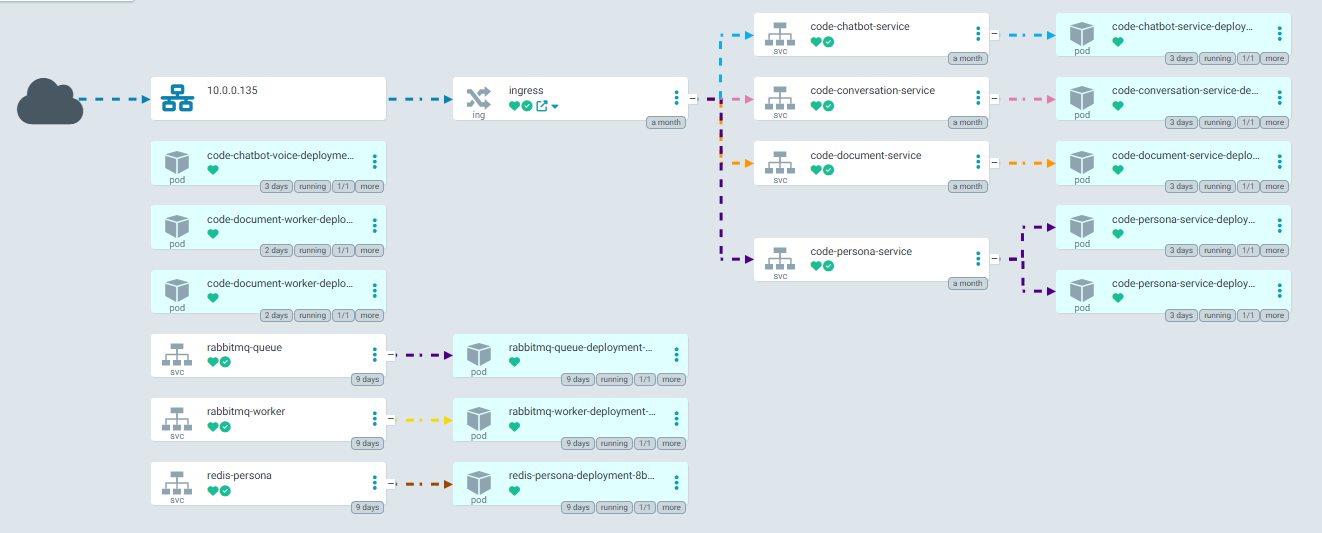
\includegraphics[width=0.95\textwidth]{pictures/argocd-web-ui.png}
\caption{Kết quả giao diện ArgoCD chạy docker trong kubernetes}
\end{figure}

\textbf{Các quyết định cấu hình Kubernetes trong kho lưu trữ GitOps của dự án này:}

\begin{itemize}
\item \textbf{Triển khai các dịch vụ trung gian trong cụm (\texttt{RabbitMQ} và \texttt{Redis}):}
Triển khai \texttt{RabbitMQ} và \texttt{Redis} cùng các dịch vụ khác trực tiếp trong cụm Kubernetes giúp tăng tốc độ xử lý, loại bỏ độ trễ mạng (network latency), không bị giới hạn tài nguyên như các gói miễn phí (ví dụ: \texttt{cloudAMQP}) và không cần gọi kết nối ra bên ngoài (\texttt{redis.io}) như dịch vụ thanh toán được triển khai ở Heroku.

\item \textbf{Cấu hình loại dịch vụ là \texttt{ClusterIP} cho các hàng đợi và bộ nhớ đệm:}
Cấu hình \texttt{RabbitMQ} queue (kết nối \texttt{conversation service} và \texttt{chatbot service}), \texttt{RabbitMQ} worker (kết nối \texttt{document service} và \texttt{document worker}) và \texttt{Redis} (lưu trữ cache của \texttt{persona service}) có loại dịch vụ (\texttt{type}) là \texttt{ClusterIP}. Thiết lập này giúp ngăn chặn hoàn toàn các client từ bên ngoài cụm Kubernetes kết nối trực tiếp đến các dịch vụ nội bộ này.

\item \textbf{Triển khai dịch vụ giọng nói (\texttt{Voice Deployment} - \texttt{LiveKit Agent}):}
Dịch vụ giọng nói không cấu hình service đi kèm. Do đó, các tài nguyên khác (cả bên trong và bên ngoài cụm Kubernetes) không thể chủ động định tuyến và gửi các yêu cầu trực tiếp vào các Pod của \texttt{voice agent}. Thay vào đó, \texttt{voice agent} hoạt động như một \texttt{LiveKit Agent} chủ động lắng nghe và kết nối trực tiếp với máy chủ \texttt{LiveKit}.

\item \textbf{Triển khai dịch vụ xử lý tài liệu (\texttt{Document Worker} - \texttt{Celery}):}
Tương tự như \texttt{voice agent}, dịch vụ \texttt{document worker} (sử dụng \texttt{Celery}) cũng không cấu hình service đi kèm. \texttt{Document worker} hoạt động theo cơ chế chủ động lắng nghe hàng đợi từ \texttt{RabbitMQ} worker để xử lý các tác vụ bất đồng bộ.

\item \textbf{Cấu hình \texttt{gRPC}:}
Dịch vụ \texttt{gRPC} chạy trên cổng \texttt{PORT 50051} nhưng được cấu hình với loại dịch vụ là \texttt{ClusterIP} và không cấu hình Ingress. Thiết lập này ngăn chặn các client bên ngoài cụm Kubernetes kết nối trực tiếp đến \texttt{gRPC}. Nhờ đó, mọi yêu cầu từ client bắt buộc phải đi qua \texttt{conversation service} để kiểm tra nghiệp vụ gói thanh toán VIP trước khi gửi đến \texttt{chatbot service}.
\end{itemize}

\begin{figure}[H]
\centering
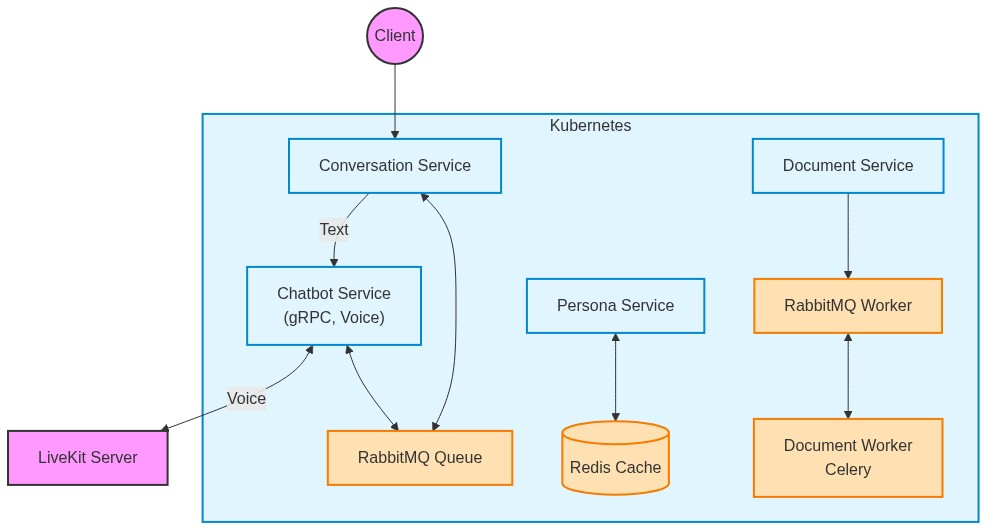
\includegraphics[width=0.95\textwidth]{pictures/Kubernetes.png}
\caption{Cấu hình Kubernetes trong kho lưu trữ GitOps của dự án}
\end{figure}

% \subsubsection{Giao tiếp giữa các services}

% {Giao tiếp trực tiếp}

% % REST persona
% % REST thanh toán gọi user

% <!-- gRPC là gì? -->
% gRPC
% webhook
% <!-- webhook cũng là giao tiếp trực tiếp (thanh toán...) -->

% % bên gửi và bên nhận phải cùng hoạt động dẫn đến phụ thuộc nhau

% % ## Gián tiếp (qua trung gian)

% % message queue :
% kafka
% RabbitMQ

% % bên gửi và bên nhận hoạt động độc lập (không cần biết địa chỉ)

% TODO: Trình bày về Outbox
